\documentclass[./writeup.tex]{subfiles}
\begin{document}
\section{Robot Vision}
\subsection{Joint State Estimation 1}
\subsubsection{Algorithm Overview}
This section explains the algorithm for estimating the robot joint angles. Two separate, supporting processes are invoked to capture the images from camera 1 (orthogonal to the y axis) and camera 2 (orthogonal to the x axis). Using both processes the joint angles are determined using vector geometry. Knowing that $a \bullet b = |a| |b| \cos \theta$ angle $\theta$ for each joint rotation can be completed by identifying the angle betweent the joint vector a and it's orthogonal counterpart $\cos^{-1}(\frac{a \bullet b}{|a| |b|})$.
\newline
\newline
The first step is determining the joint location vectors from the images. This was completed by using colour masking techniques to isolate the joints from the rest of the image. The center of each joint was estimated by calculating the X, Y moments of each binary image that was derived from the colour masking, which gave co-ordinates in pixel space. If this process failed due to camera obscufication then the co-ordinates captured by the previous successful image capture were used as a proxy for the joint location. Figure one provides some examples of this happening.
\begin{figure}[h!]
    \centering
    \subfloat[Example of obscufication of the end effector and partial obscufication of joint 3 in the x frame.]{\label{b}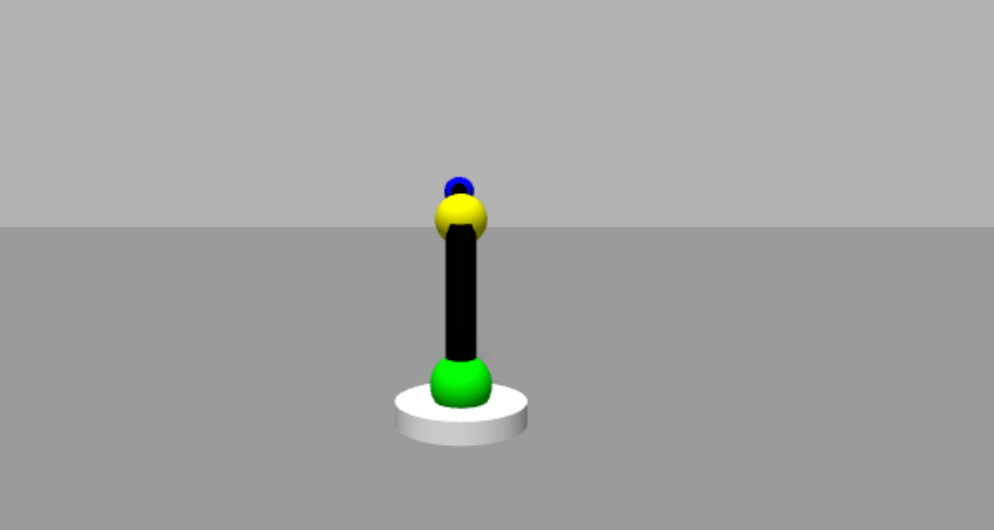
\includegraphics[width=.45\linewidth]{x_yellow_fail.png}}\hfill
    \subfloat[Example of obscufication of joint 3 in the y frame.]{\label{c}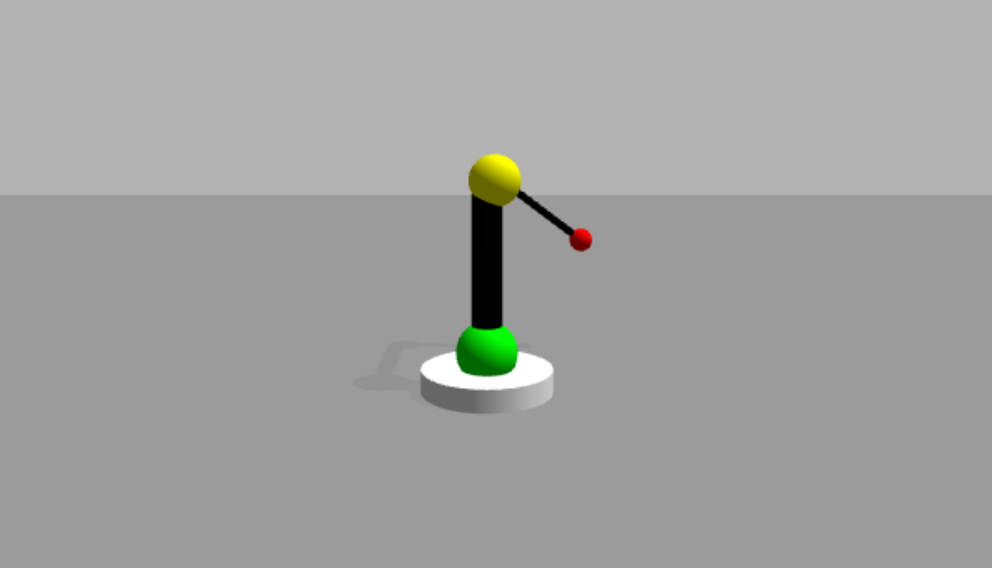
\includegraphics[width=.45\linewidth]{y_blue_fail.png}}
    \caption{Examples of where joint detection would fail. When this happens the last previous joint recording was used in the algorithm.}
\end{figure}
Camera one tracks co-ordinates x and z, and camera two tracks co-ordinates y and z. Using this information the 3d location of the joint is estimated by taking the x and y co-ordinates from each camera, with the z co-ordinate being the average of the z co-ordinate returned by the two cameras. This gives a 3 dimensional vector spanning the $[X_0, Y_0, (X_1 + X_1)/2]$ space containing the location of each joint.
\newline
\newline
To identify the location of each joint it was subtracted from it's downstream equivalent (blue was subtracted from yellow and red subtracted from blue), and converted to meter basis via the following equation: $[X', Y', Z'] = [X, Y, Z] * (L / \sqrt{\sum_c \in {x, y, z} (x_i -  x_{i-1})^{2}}$. L represents the lengh of the links between joints and coord i and coord i-1 is the upstream and downstream joint. Following the meter conversion the joint angles were determined according to slightly different formulaes as demonstrated below:
\begin{itemize}
    \item \textbf{JOINT 2}: Tracks changes in the y axis between the yellow and blue joints. Because of this the scaled joint location is projected onto the identity x axis to find vector that is orthogonal to the x axis and joint 2. Joint 2 angle can be calculated as the angle between this projection and the y co-ordinate basis: $\cos^{-1} (\frac{PROJ \bullet [0, 1, 0]}{|PROJ| * |[0, 1, 0]|})$
    \item \textbf{JOINT 3}: Tracks changes in the x axis between the yellow and blue joints. Because of this the scaled joint location is projected onto the identity y axis to find vector that is orthogonal to the y axis and joint 2. Joint 3 angle can be calculated as the angle between this projection and the x co-ordinate basis: $\cos^{-1} (\frac{PROJ \bullet [1, 0, 0]}{|PROJ| * |[1, 0, 0]|}) - \pi$
    \item \textbf{JOINT 4}. Tracks the difference between the end effector and the blue joint in the y axis. As we're seeking the angle between these two vectors no projection onto the identity co-ordinate system is needed and the angle is $\cos{-1}(\frac{R \bullet Y}{|R| * |Y|})$
\end{itemize}
The inverse cosine implementation used is the numpy \textbf{arccos} method. As this does not take into consideration the signage of the vectors whether the rotation is positive or negative is calculated by reviewing the joint locations. For joints 2 and 4, in pixel basis, if the upstream x co-ordinate is to the left of it's downstream joint then we know a negative rotation has occured and the angle is multiplied by -1 to reflect this fact. A similar process is taken by looking at the y co-ordinate for changes to the x axis for joint 3.
\subsubsection{Results}
The algorithm was ran for 120 seconds with the recorded change in joint angle plotted against the estimated change in joint angle from the vision algorithm. Separate graphs are used to plot the deltas between the joint angles and the vision algorithm estimations. The results are shown in the plots below:
\begin{figure}[h!]
\centering
\subfloat[Plot Comparing Changes to Joint 2 Against Baseline]{\label{Figure A}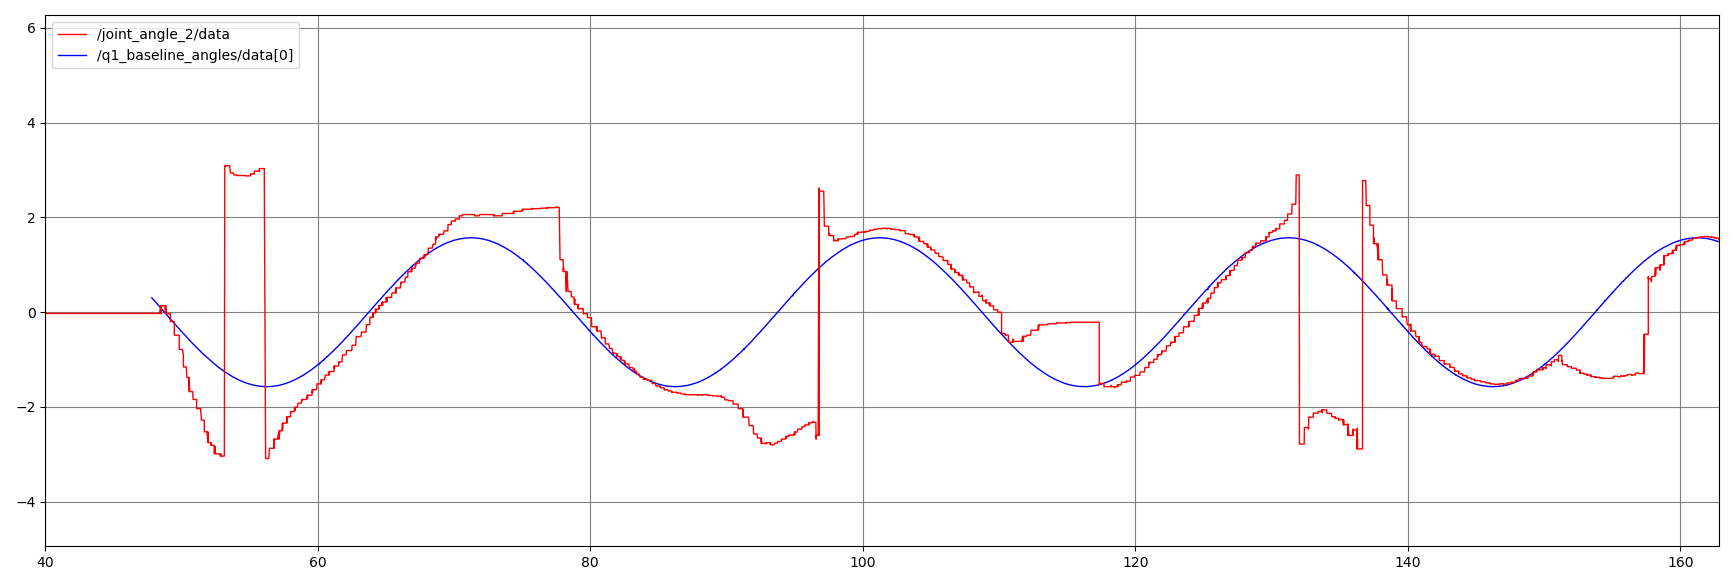
\includegraphics[width=.45\linewidth]{ja_2.png}}\hfill
\subfloat[Plot Comparing Changes to Joint 3 Against Baseline]{\label{b}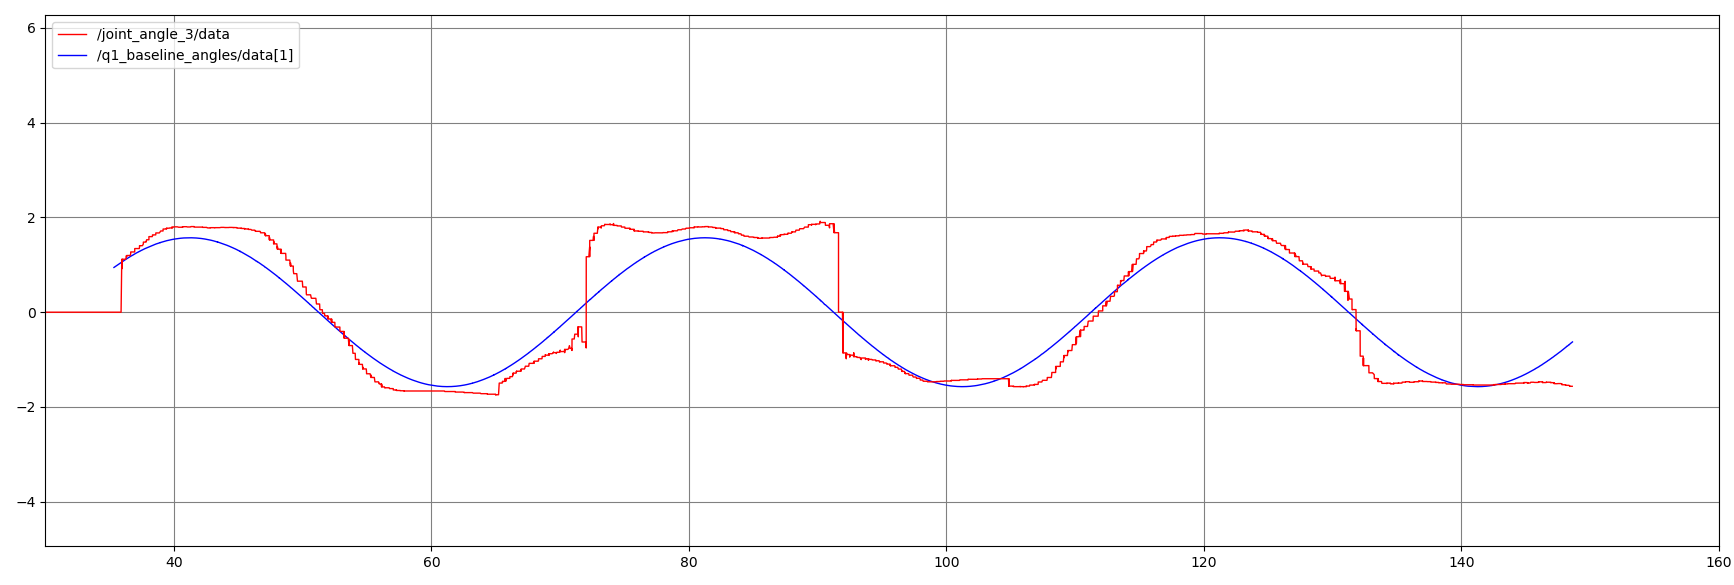
\includegraphics[width=.45\linewidth]{ja_3.png}}\hfill
\subfloat[Plot Comparing Changes to Joint 4 Against Baseline]{\label{c}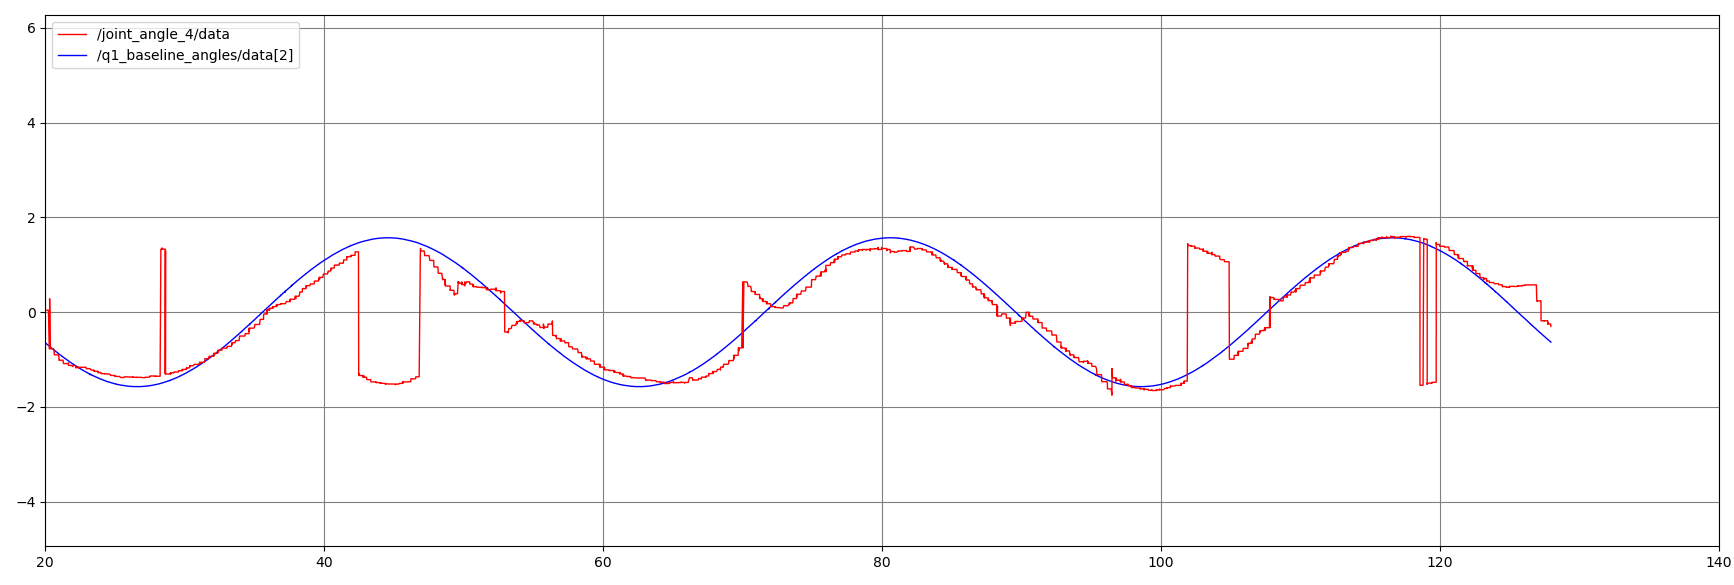
\includegraphics[width=.45\linewidth]{ja_4.png}}
\caption{The x axis denotes the algorithm run-time in float seconds. The y axis is used to plot the degrees in radians of rotation for each joint. The red curve is the estimated joint angle and the blue curve is the baseline joint angle.}
\end{figure}
\subsubsection{Discussion}
The joint angle detection algorithm is reasonable effective at tracking the changes to the joint states. For all the joints measured the velocities recorded by the algorithm roughly follow a sinusodial signal that's aligned with the changes to the joint angles.
\newline
\newline
The most accurate tracking occurs at joint 3. Whether this accuracy is a product of there only being one rotation on the x axis would require further empirical investigation but it's a useful starting explanation.
\newline
\newline
When the velocities of the joints 2 and 4 reach a maxima and minima the performance of the algorithm begins to deterorate. The most likely reason for this that when the joints these configurations the cameras are unable to gain a clear view of the joints and the previous measurements are used. This results in larger error between the baseline and the calculated joint angles. In figures 1a and 1c sharp increases in error are seen at the maxima and minima of the baseline sine waves. It is at these points that the algorithm cannot identify the joints due to there being a limited picture of the joints or no picture at all. This observation is supported by the fact that over the 120 second period the algorithm failed to isolate the joints 292 times on the y axis, whereas 11 failures occured on the x axis.
\newline
\newline
As the number of processes that change joint angles on a particular axis increases the algorithm performance deterorates. This is because the combined processes put the joints into configurations that make colour detection difficult, which prevents the algorithm from identifying the joint locations and angles.
\subsection{Joint State Estimation 2}
\subsubsection{Algorithm Overview}
This section describes the algorithm for measuring the joint angles when joints 1, 3 and 4 are rotated according to sinusodial waves. The colour thresholding techniques and scaling steps described in question 2 to isolate the joints and determine their locations in meter space were reused for this section.
\newline
\newline
The only changes made was the projection logic to determine the joint angles. The joints follow a Z, X, Y rotation. Although the Z rotation is a product of rotating the green joint, rotations in the z axis lead to changes in the blue joint. Thus rotations on the z axis of joint 1 are estimated based on changes captured in the y axis to joint 3. Knowing that there rotations on the X axis were held constant, the joint angles were determined according to the below formulaes:
\begin{itemize}
    \item \textbf{JOINT 1}: The 3D co-ordinates of the blue joint was projected onto an 2D X, Y plane with the angle measured against the Y basis co-ordinate system: $\cos^{-1}(\frac{[BLUE_x, BLUE_y] \bullet [0, 1] }{|[BLUE_x, BLUE_y]| * |[0, 1]|})$. Whether a positive or negative rotation has occured is estimated by looking at whether the blue joint's y co-ordinate is to the right of the yellow joint.
    \item \textbf{JOINT 3}: Joint 3 is the rotation of blue joint on the y axis. This is represented by a combined rotation of Z and Y the angle between the blue vector and the z co-ordinate system is measured: $\cos^{-1}(\frac{BLUE \bullet [0, 0, 1]}{|BLUE| * |[0, 0, 1]})$. Whether a positive or negative rotation has occured is estimated by looking at whether the blue joint's x co-ordinate is to the right of the yellow joint.
    \item \textbf{JOINT 4}: Joint 4 is based on the angle of the projection of the red joint onto the red blue joint. If the location of the red y co-ordinate is to the right of the blue co-ordinate then we predict that a negative rotation has occured: $\cos^{-1}(\frac{RED \bullet BLUE}{|RED|*|BLUE|})$
\end{itemize}
\subsubsection{Results}
The figure below plots the predicted joint angle changes from the cameras against the baseline joint angle changes:
\begin{figure}[h!]
    \centering
    \subfloat[Plot Comparing Changes to Joint 1 Against Baseline]{\label{Figure A}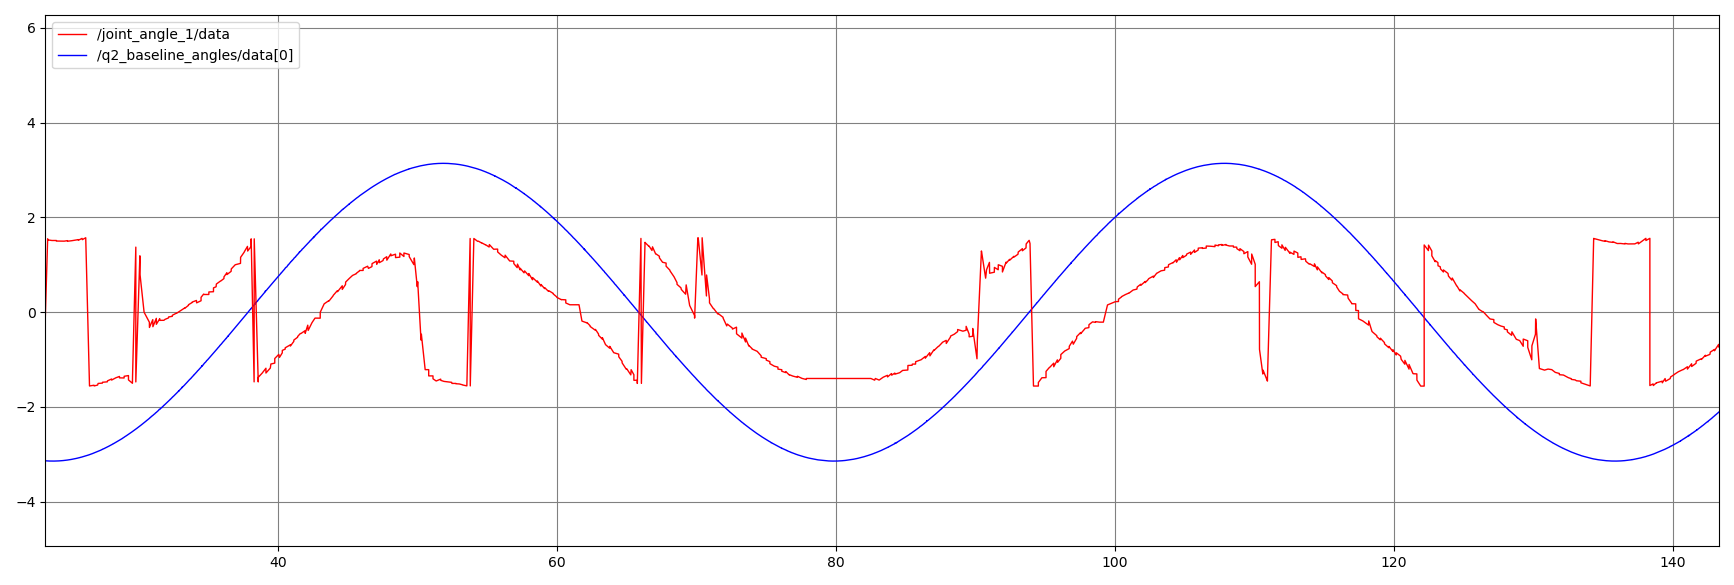
\includegraphics[width=.45\linewidth]{ja1_q1.png}}\hfill
\subfloat[Plot Coeparing Changes to Joint 3 Against Baseline]{\label{b}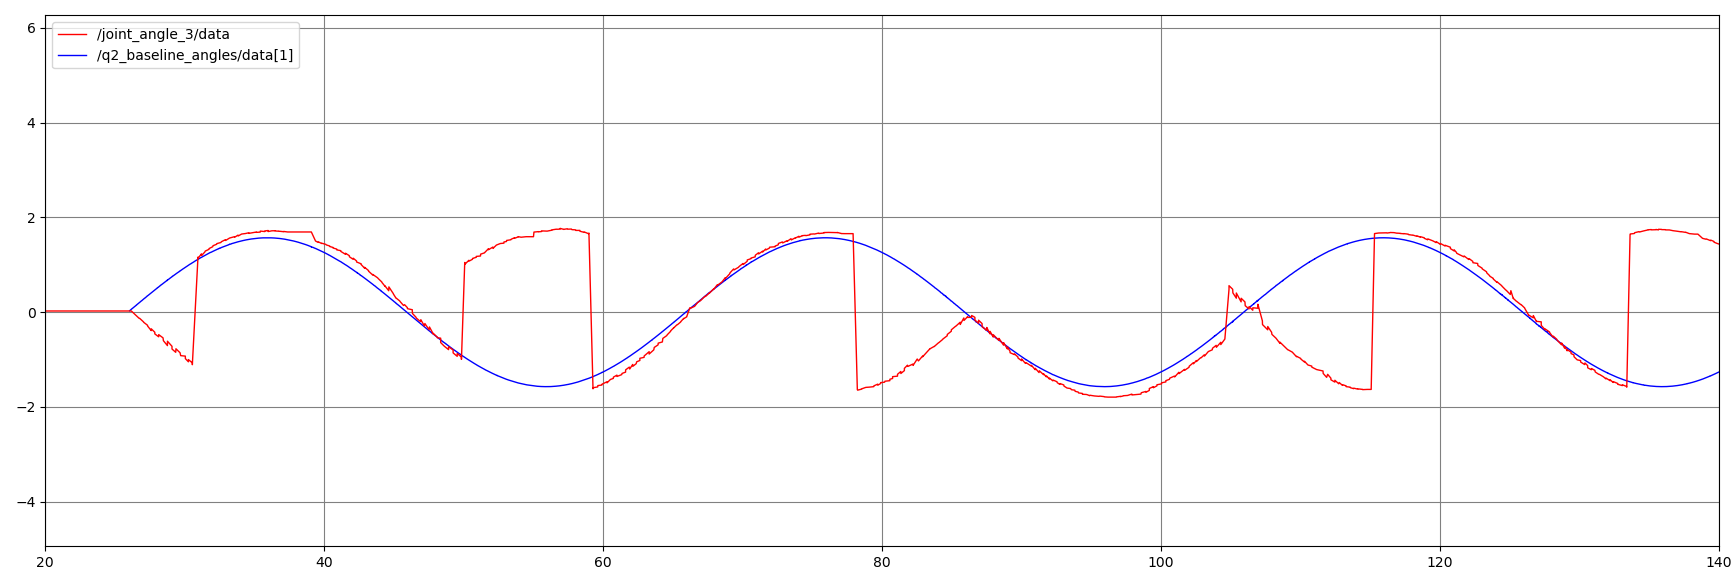
\includegraphics[width=.45\linewidth]{ja3_q2.png}}\hfill
    \subfloat[Plot Comparing Changes to Joint 4 Against Baseline]{\label{c}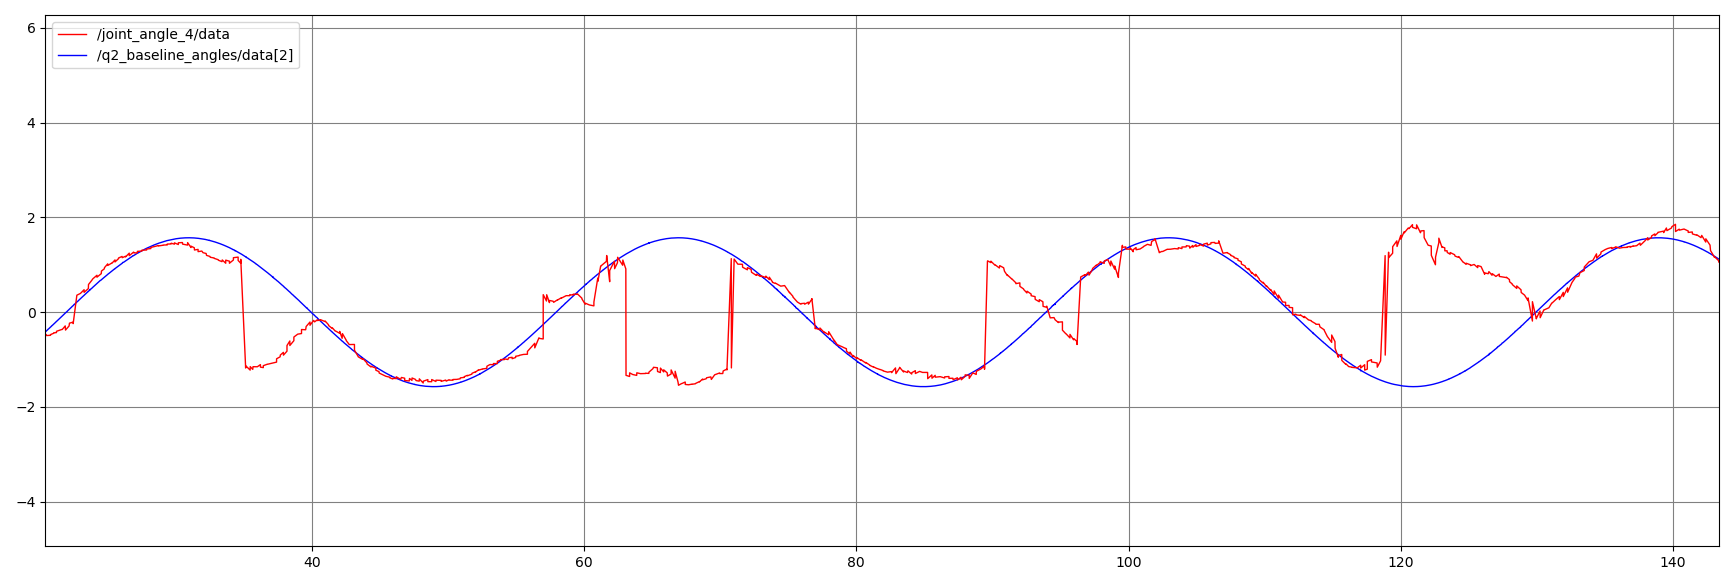
\includegraphics[width=.45\linewidth]{ja4_q2.png}}
\end{figure}
\section{Robotics}
\subsection{Forward Kinematics}
\subsubsection{Methods}
This section briefly describes the equation used to calculate the location of the end effector through forward kinematics. Based on the fact that the x axis is orthogonal to the z axis and intersects with the x axis the Devanit-Hartenberg homogenous transformation method is used to calculate each rotation and displacement \cite{SPONG2020}.
\newline
\newline
The matrices are parametirized with the following table that follow the Devanit-Hatenberg conventions. For the first link there is a constant displacement of 4 according to the z axis and because the links start in a co-ordinate system where x, y, z are orthogonal there is no initial rotation.
\newline
\newline
Links three and 4 include a constant displacement in the X direction of 3.2 and 2.8 and a rotation about their respective X and Y axis. To compensate for the inital transformation in the z direction the rotation matrix starts in the Z direction for both co-ordinate frames so includes a 90 degree (approximately pi/2) rotation.
\begin{table}[h!]
    \centering
    \begin{tabular}{llll}
    theta (rotation z) & alpha (rotation x) & ALPHA (displacement x) & d (displacement z)  \\
    theta              & 0                  & 0                      & 4                   \\
    90 (pi/2 radians)  & alpha              & 3.2                    & 0                   \\
    90 (pi/2 radians)  & alpha              & 2.8                    & 0                   \\
    \end{tabular}
\end{table}
\newline
\newline
The resultant forward kinematics equation returned is derived by the following matrix multiplication. $\theta_1, \theta_2, \theta_3$ represent the different joint angles:
\newline
\newline
$ \begin{bmatrix}
    cos(\theta_1) & 0 & sin(\theta_1) & 0 \\
    sin(\theta_1) & cos(\theta_1) & -cos(\theta_1) & 0 \\
    0 & 1 & 0 & 4 \\
    0 & 0 & 0 & 1
\end{bmatrix}
\bullet
\begin{bmatrix}
    0 & -cos(theta_2) & sin(theta_2) & 3.2 \\
    1 & 0 & 0 & 0 \\
    0 & sin(theta_2) & cos(theta_2) & 0 \\
    0 & 0 & 0 & 1
\end{bmatrix}
\bullet
$
\newline
\newline
$
\begin{bmatrix}
    0 & -cos(theta_3) & sin(theta_3) & 2.8 \\
    1 & 0 & 0 & 0 \\
    0 & sin(theta_3) & cos(theta_3) & 0 \\
    0 & 0 & 0 & 1
\end{bmatrix}$
\subsubsection{Results}
The table below demonstrates the predictions from the forward kinematics equation against the expected results. Given the limited accuracy of the angle detection algorithm for joints 1, 3 and 4 a high source of error is not surprising. The fact that predicted z is a constant combination of the first two links demonstrates that there is an error in the forward kinematics calculation. This error is likely in the identification of the initial co-ordinate matrices and default rotations around the x and y axis for the second and third matrices.
\newline
\newline
\begin{tabular}{rrrrrr}
    \toprule
     expected\_x &  expected\_y &  expected\_z &  predicted\_x &  predicted\_y &  predicted\_z \\
    \midrule
          4.159 &      -4.969 &       7.616 &     2.287 &     3.061 &       7.2 \\
          2.411 &      -1.413 &       9.602 &    -0.580 &     5.039 &       7.2 \\
         -5.992 &      -1.872 &       7.784 &    -1.847 &     0.810 &       7.2 \\
         -3.828 &      -6.632 &       6.432 &    -2.608 &     2.535 &       7.2 \\
         -1.930 &      -0.386 &       9.804 &    -0.934 &    -1.945 &       7.2 \\
          5.263 &      -0.658 &       8.477 &    -0.409 &     0.230 &       7.2 \\
          3.294 &      -0.630 &       9.421 &    -2.603 &     4.109 &       7.2 \\
          1.766 &      -2.698 &       9.466 &    -1.609 &     5.485 &       7.2 \\
         -1.304 &      -7.513 &       6.469 &     2.644 &     1.831 &       7.2 \\
          3.475 &       3.475 &       8.709 &    -0.421 &     0.075 &       7.2 \\
    \bottomrule
\end{tabular}
\end{document}